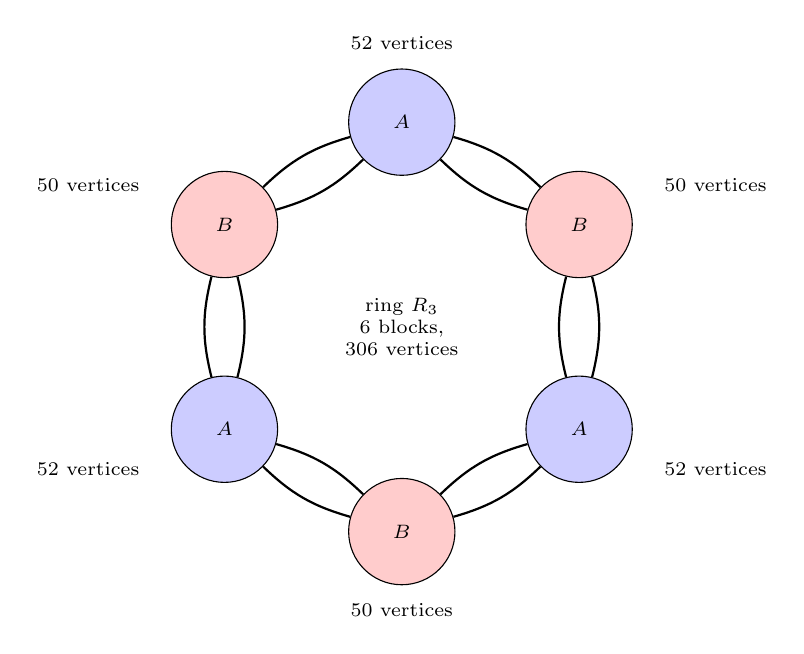
\begin{tikzpicture}[every node/.style={font=\scriptsize}]
\node[draw,circle,minimum size=1.35cm,fill=blue!20] (b0) at (0.000,2.600) {$A$};
\node at (0.000,3.600) {52 vertices};
\node[draw,circle,minimum size=1.35cm,fill=red!20] (b1) at (2.252,1.300) {$B$};
\node at (3.984,1.800) {50 vertices};
\node[draw,circle,minimum size=1.35cm,fill=blue!20] (b2) at (2.252,-1.300) {$A$};
\node at (3.984,-1.800) {52 vertices};
\node[draw,circle,minimum size=1.35cm,fill=red!20] (b3) at (0.000,-2.600) {$B$};
\node at (0.000,-3.600) {50 vertices};
\node[draw,circle,minimum size=1.35cm,fill=blue!20] (b4) at (-2.252,-1.300) {$A$};
\node at (-3.984,-1.800) {52 vertices};
\node[draw,circle,minimum size=1.35cm,fill=red!20] (b5) at (-2.252,1.300) {$B$};
\node at (-3.984,1.800) {50 vertices};
\draw[thick,bend left=14] (b0) to (b1);
\draw[thick,bend right=14] (b0) to (b1);
\draw[thick,bend left=14] (b1) to (b2);
\draw[thick,bend right=14] (b1) to (b2);
\draw[thick,bend left=14] (b2) to (b3);
\draw[thick,bend right=14] (b2) to (b3);
\draw[thick,bend left=14] (b3) to (b4);
\draw[thick,bend right=14] (b3) to (b4);
\draw[thick,bend left=14] (b4) to (b5);
\draw[thick,bend right=14] (b4) to (b5);
\draw[thick,bend left=14] (b5) to (b0);
\draw[thick,bend right=14] (b5) to (b0);
\node[align=center] at (0,0) {ring $R_3$\\ $6$ blocks,\\ 306 vertices};
\end{tikzpicture}
